\chapter{Progetto}
\label{progetto}

In questo capitolo si propone il progetto realizzato per raggiungere gli obiettivi preposti: si è partiti dalla realizzazione di un classificatore basato su \textit{Random Forest} per poi passare ad una versione più elaborata, utilizzando un \textit{Multilayer Perceptron}. Il passo successivo ha riguardato la creazione di una \textit{Generative Adversarial Network} a partire da un \textit{Autoencoder} in grado di rafforzare un classificatore generando domini sintetici


\section{Classificatore Random Forest}
\label{randomforest}
La prima fase di questo studio è stata quella di implementare un classificatore in grado di separare efficacemente domini \textit{DGA} da domini non malevoli basandosi unicamente sulle caratteristiche linguistiche dei domini: infatti, ad un esame preliminare, i domini \textit{DGA} presentano caratteristiche ben differenti da semplici frasi o parole che solitamente compongono i domini reali.

Si è scelto di utilizzare Random Forest in quanto ritenuto il più adatto al caso in esame. L'algoritmo è stato inoltre messo a confronto con \textit{Support Vector Machine} e \textit{Naive-Bayes}. \todo{indicare SVM e GNB solo nei risultati?}

All'interno del classificatore \textit{Random Forest} \cite{randomforest}, ogni albero dell'insieme è costruito a partire da un campione estratto con sostituzione dal \textit{training set}. In aggiunta, al momento della divisione del nodo durante la costruzione di un albero, la divisione scelta non è più la migliore soluzione tra tutte le \textit{features}. Al suo posto, la divisone che viene scelta è la migliore divisione all'interno di un \textit{subset} casuale tra tutte le \textit{features}. Come risultato di questa casualità, il \textit{bias} della foresta di solito aumenta leggermente (rispetto al \textit{bias} di un singolo albero non casuale) ma, a causa della media, la sua varianza diminuisce, di solito compensando l'aumento di \textit{bias}, quindi dando un modello generale migliore.

\subsection{Dataset}
\label{randomforestdataset}
I \textit{dataset} di \textit{training} e \textit{testing} sono stati ricavati due fonti differenti: per quel che riguarda i domini reali si è fatto riferimento alla classifica dei domini più visitati al mondo fornita da \textit{Alexa Internet Inc.} \cite{amazon:alexa} , per un totale di 1 milione di siti realmente esistenti; mentre grazie al repository fornito da \cite{github:dgarepo} è stato possibile ottenere un \textit{dataset} esaustivo di esempi \textit{DGA} da diverse famiglie di \textit{malware}. In particolare le famiglie di malware utilizzate per il training sono state: \todo{famiglie malware}

\todo{mostrare tabella esempio diversi DGA}

A partire da tale \textit{dataset} combinato si è proceduto alla creazione di un classificatore binario che fosse in grado di distinguere domini reali da domini generati algoritmicamente. 

Il passo seguente  stato creare una serie di \textit{features} che fossero in grado di descrivere le caratteristiche linguistiche dei domini presi in esame.

\todo{descrivere distribuzione caratteri Alexa vs dga}

Per raggiungere tale obiettivo si è fatto riferimento a ricerche già esistenti: \cite{180232} \cite{Yadav:2010:DAG:1879141.1879148} \cite{Yadav:2012:DAG:2428696.2428722} \cite{Schiavoni2014}. Di seguito viene illustrato l'insieme di tali \textit{features}:

\subsection{Features}
\label{randomforestinterno}

\begin{itemize}

\item \textbf{Rapporto tra caratteri significativi}. Modella il rapporto dei caratteri della stringa $p$ che formano una parola significativa all'interno del dizionario Inglese. Un valore basso indica la presenza di algoritmi automatici. In dettaglio, si divide $p$ in $n$ sotto-parole significative $w_i$ di almeno $3$ caratteri: $|wi| \ge 3$ cercando di lasciare fuori meno caratteri possibili: $$R(d) = R(p) = \frac{max(\sum_{i=1}^n |wi|)}{\left | p \right |}$$ 
Se $p = \text{facebook}$, $R(p) = \frac{(|\text{face}| + |\text{book}|)}{8} = 1$ allora il dominio è composto completamente da parole significative, mentre $p = \text{pub03str}$, $R(p) = \frac{|\text{pub}|}{8} = 0.375$. 

    

\item \textbf{Punteggio di normalità degli n-grammi}: Questa classe di \textit{features} modella la pronunciabilità di un nome di dominio rispetto la lingua Inglese. Più la combinazione di fonemi del dominio è presente  all'interno del Dizionario Inglese più tale dominio è pronunciabile. Domini con un basso numero di tali combinazioni sono probabilmente generati algoritmicamente. Il calcolo avviene estraendo lo n-gramma di $p$ di lunghezza $n \in \left \{1, 2, 3, 4, 5 \right \}$ e contando il numero di occorrenze di tale n-gramma all'interno del Dizionario Inglese. Tali \textit{features} sono quindi parametriche rispetto ad n: 
$$S_n(d) = S_n(p) \:= \frac{\sum_{\text{n-gramma t in p}} count(t)}{\left | p \right | - n + 1}$$ 
dove $count(t)$ sono le occorrenze dello n-gramma nel dizionario. Ad esempio $S_2(facebook) = fa_{109} + ac_{343} + ce_{438} + eb_{29} + bo_{118} + oo_{114} + ok_{45} = 170.8$

       
\item \textbf{Rapporto tra caratteri numerici} Questa \textit{feature} rappresenta il rapporto tra i caratteri numerici presenti all'interno del nome di dominio rispetto la lunghezza totale della parola. Molte famiglie di \textit{malware} utilizzano \textit{DGA} che generano domini tramite una distribuzione uniforme di caratteri alfabetici minuscoli e numeri, questo porta a domini generati algoritmicamente che presentano una maggior presenza di numeri al loro interno rispetto ai domini reali.


\item \textbf{Rapporto tra vocali e consonanti} Questa \textit{feature} modella il rapporto tra vocali e consonanti all'interno del nome di dominio.


\item \textbf{Lunghezza del nome di dominio} Questa \textit{feature} calcola la lunghezza del dominio. Molte famiglie di \textit{malware} utilizzano \textit{DGA} che generano domini di lunghezza costante, generalmente molto lunghi rispetto ai domini reali.
	
\end{itemize}

L'implementazione di tali \textit{features} ha permesso di ottenere un \textit{dataset} in grado di modellare le caratteristiche linguistiche dei nomi di dominio mostrati al capitolo \ref{randomforestdataset}. Da tale spunto è partita la fase iniziale di \textit{testing} 

\subsection{Output}
\label{randomforestoutput}
L'obiettivo di tale classificatore è quello di riuscire a separare in maniera efficace i domini reali da quelli generati algoritmicamente. A tale proposito ???
\todo{ampliare questa sezione e chiedere a Marchetti}
\todo{indicare il capitolo coi risultati di Random Forest} 

Durante la fase di sperimentazione il classificatore si è rivelato efficace rispetto la maggior parte delle famiglie di \textit{DGA}. Il caso particolare della famiglia \textit{suppobox} \cite{geffner2013end} ha messo in particolare difficoltà il classificatore in quanto tale algoritmo genera domini in maniera pseudo-casuale, concatenando due parole a partire da un \textit{subset} del dizionario inglese di 384 parole. Tale caratteristica fa si che le \textit{features} linguistiche estratte da questa famiglia di \textit{malware} siano molto simili a quelle presenti nei domini reali.

\todo{mostrare esempio suppobox}

\todo{???????????????????}

A partire da questo risultato si scelto di procedere con la progettazione di un classificatore neurale in grado di superare tale problematica.


\section{Classificatore Neurale}
\label{classificatorenn}
Questo classificatore neurale nasce con l'intento di superare le difficoltà incontrate dal precedente classificatore basato su \textit{Random Forest}, utilizzando le caratteristiche delle reti neurali, in grado di estrarre \textit{features} a partire dai dati grezzi. Si è scelto di partire dall'architettura di tipo \textit{Multilayer Perceptron} con l'obiettivo di ottenere risultati migliori rispetto al caso mostrato nella sezione precedente.

I passi del progetto sono stati la codificazione dei domini in valori numerici, l'individuazione di una architettura ottimale per classificare i dati in esame ed un'ultima fase di \textit{tuning} degli iperparametri della rete neurale. 

\subsection{Input}
\label{classificatorenninput}
A partire dal \textit{dataset} creato per il precedente caso, si è deciso di convertire direttamente i nomi di dominio alfanumerici in vettori numerici, mappati secondo il dizionario di tutti i caratteri ammessi \cite{icann} (lettere minuscole a-z, numeri 0-9, tratto d'unione "-" ). L'obiettivo è quello di fornire al classificatore neurale in questione una rappresentazione il più possibile aderente ai dati reali, senza l'ausilio di \textit{features} ingegnerizzate a priori, lasciando così la libertà alla rete neurale di estrarre le caratteristiche più appropriate per la distinzione dei domini. Come scelta progettuale si è deciso di limitare la dimensione dei domini a 15 caratteri per ognuno, in modo da ottenere un \textit{dataset} di dimensioni fissate e sopperire alle differenti lunghezze di ogni dominio tramite un semplice \textit{padding} di zeri in testa ad ogni stringa codificata.

Assieme ai dati codificati è stato generato un vettore di \textit{target} nel quale viene indicato da 0 o da 1 se il dominio in esame è di tipo reale o generato algoritmicamente. L'obiettivo quindi è di attuare un classificatore binario in grado di prevedere correttamente a quale categoria appartiene un dominio esaminato 

\subsection{Architettura}
\label{classificatorenninterno}
L'architettura scelta in prima fase è stata quella del \textit{Multilayer Perceptron} \textit{(abbr. MLP)}, una tipologia di rete neurale \textit{feedforward} tipicamente formata da almeno tre livelli di nodi. Ad esclusione del livello di \textit{input} i livelli del MLP utilizzano  funzioni di attivazione non lineari che permettono di eseguire distinzioni tra dati non linearmente separabili. Considerando una rete formata da $m$ neuroni,  se si considera $d$ come numero di input, si avrà il seguente output
$$y_j=y\left( \sum_{i=0}^d w_{ji}x_i \right)$$

nel quale $x_i$ sono gli input e $w_{ji}$ sono i pesi di ogni input combinati con ogni output. 

\todo{aggiungere ed estendere la teoria MLP nel capitolo precedente?}

Nel caso in esame è stata utilizzata per i livelli interni la funzione di attivazione \textit{Rectifier Linear Unit} (ReLU) \cite{relu} definita dalla funzione 
$$f(x) = x^+ = max(0,x)$$
\todo{inserire grafo ReLU}
dove $x$ rappresenta l'\textit{input} del neurone. 
I vantaggi di tale funzione sono una migliorata \textit{performance} rispetto ad altre funzioni similari come \textit{tanh} e \textit{sigmoid} per quel che riguarda la convergenza della discesa stocastica del gradiente. 

Per quel che riguarda la funzione di attivazione del livello di \textit{output} si è scelta la funzione \textit{sigmoidea}, definita dalla formula 
$$P(t) = \frac{1}{1+e^{-t}}$$
\todo{inserire grafo sigmoid}

La struttura finale del \textit{MLP} in esame è stata raggiunta dopo una serie di test sperimentali in cui si sono messi a confronto tre modelli differenti di per numero di neuroni all'interno degli \textit{hidden layer}: 
\begin{itemize}
\item un modello ridotto composto da un layer di input con un numero di neuroni pari alla dimensione delle stringhe codificate, un layer intermedio di dimensione dimezzata rispetto al precedente ed il layer finale di uscita di dimensione 1 per attuare la classificazione binaria, oggetto di studio.

\item un modello allargato composto da un layer di input con un numero di neuroni pari alla dimensione delle stringhe codificate, due layer intermedi di dimensioni moltiplicate di diversi ordini rispetto al layer iniziale ed un layer finale di dimensione 1.

\item un modello intermedio composto da un layer di input con un numero di neuroni pari alla dimensione delle stringhe codificate, un layer intermedio di dimensione 128, un layer di dimensione minore a 64 ed un layer finale di dimensione 1. (Figura \ref{fig:pieraz})

\end{itemize}

I tre modelli messi a confronto hanno mostrato risultati simili, tuttavia  il modello intermedio si è dimostrato più performante, con un costo computazionale irrisorio rispetto al modello allargato, pertanto è stato scelto come riferimento per gli studi successivi.

\begin{figure}[htb]
    \centering
    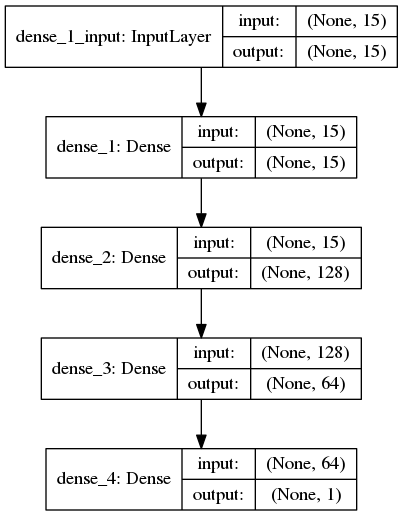
\includegraphics[width=.4\columnwidth]{figures/pieraz_baseline.png}
    \caption{Grafico del modello intermedio. Escluso il layer di input iniziale, si notino gli \textit{hidden layer} dense2 e dense3 di dimensioni rispettivamente 128 e 64 }
\label{fig:pieraz}
\end{figure}

\subsection{Output}
\label{classificatorennoutput}
L'intento della rete neurale proposta è quello di classificare autonomamente domini reali da domini generati algoritmicamente, con l'obiettivo di superare le fragilità del classificatore precedente (\ref{randomforest}) ed avere una linea di confronto affidabile per lo \textit{step} di lavoro successivo: l'introduzione di un sistema di \textit{adversarial learning} che possa rafforzare tale classificatore. 
\todo{come ampliare??????????????}

\subsection{Realizzazione Adversarial Learning}
\label{adv}
Ricerche precedenti hanno dimostrato che molti modelli di machine learning, incluse le reti neurali, sono vulnerabili agli \textit{adversarial examples} \cite{1312.6199},  \cite{1412.6572} . In particolare la ricerca proposta in \cite{1412.6572} introduce il metodo del \textit{fast gradient sign} per scoprire \textit{adversarial examples} perturbando un campione noto $x$ con una piccola quantità $\Delta x =  \in sign(\nabla_x J(\theta,x,y))$ dove $\theta$ rappresenta i parametri del modello e $J$ il costo necessario a classificare $x$ come $y$.
Separatamente \cite{1406.2661} propone l'uso di \textit{Generative Adversarial Network (abbr. GAN})  come \textit{framework} in grado di generare campioni artificiali provenienti dalla stessa distribuzione del training set.
Le GAN incorporano due modelli: un generatore ed un discriminatore i quali competono in una serie di turni antagonisti. All'interno del contesto del lavoro presentato in questo elaborato, il generatore impara a creare nuovi domini artificiali mentre il discriminatore impara a distinguere tali domini artificiali da quelli reali. L'intento di tale lavoro è usare la GAN per produrre domini artificiali realistici e di conseguenza incrementare la precisione del classificatore presentato nella sezione precedente attraverso l'\textit{adversarial training}.

\section{Autoencoder}
\label{autoencoder}
Il punto di partenza per il lavoro di progettazione di una \textit{GAN} è stato l'implementazione di un \textit{Autoencoder} funzionante.  Un \textit{Autoencoder} è un modello di rete neurale non supervisionata con lo scopo di riprodurre il proprio input passando attraverso una rappresentazione codificata, generalmente a dimensione inferiore \cite{MAL-006} \cite{Liou:2008:MWP:1411851.1412074}. Si supponga di avere un set di training $\left\{ x^{(1)}, x^{(2)}, x^{(3)}, \ldots \right\}$ dove $x^{(i)} \in \mathbb{R}^n$. L'obiettivo di un autoencoder generico è $y^{(i)} = x^{(i)}$ cercando di imparare una funzione che approssima x $h_{W,b}(x) \approx x$. Un \textit{autoencoder} tipicamente consiste in due macro-componenti:
\begin{itemize}
\item funzione \textbf{Encoder} $h = f(x)$ la quale trasforma l'input una rappresentazione codificata (generalmente a dimensione minore)
\item funzione \textbf{Decoder} $r = g(h)$ in grado di ricostruire l'input a partire dalla rappresentazione codificata. 
\end{itemize}

Tuttavia il reale obiettivo di un \textit{autoencoder }non è quello di imparare perfettamente a riprodurre l'input fornito (in quanto sarebbe un'operazione priva di utilità), bensì vengono introdotti vincoli che ne limitano la capacità di riproduzione ad una sola approssimazione dei dati di ingresso. Grazie a tali vincoli il modello è obbligato a dare priorità agli aspetti fondamentali dell'input, imparandone le proprietà principali. L'obiettivo di tale implementazione nel contesto di questo elaborato è poter cogliere le caratteristiche fondamentali che compongono i domini reali, per poterli riprodurre al meglio all'interno della \textit{GAN} e generare domini simili a quelli reali a partire da rumore casuale.

\subsection{Dataset Autoencoder}
\label{datasetautoencoder}
Il \textit{dataset} utilizzato per il training di tale \textit{autoencoder} è lo stesso mostrato nella sezione \ref{classificatorenninput}, in cui i domini sono mappati in vettori numerici, secondo il dizionario di caratteri ammissibili per i domini. Durante la fase di implementazione si è reso necessario un ulteriore \textit{step} di \textit{preprocessing}: i domini codificati in sequenze di valori interi sono stati ulteriormente codificati tramite il \textit{one hot encoding} \cite{onehot} in modo da formare un tensore 2D per ogni dominio, in cui ogni riga è formata da sequenze di bit a 0 tranne il carattere nella posizione indicata dal dizionario, il quale è indicato ad 1.

\todo{inserire tabella di esempio.}

Questo ulteriore passaggio è diventato necessario durante l'implementazione della \textit{GAN}, in modo da poter utilizzare il tensore di output del \textit{decoder} come ingresso per l'\textit{encoder}.


\subsection{Architettura Autoencoder}
\label{archautoencoder}
L'architettura dell'\textit{encoder} in esame è lascamente ispirata al lavoro mostrato in \cite{1508.06615} mentre il \textit{decoder} è approssimativamente una immagine speculare dell'\textit{encoder}.

Si indichi $\mathbb{V}$ come il set di caratteri validi per i domini di rete; l'\textit{encoder } contiene un primo livello di Embedding nel quale viene  imparata una mappatura lineare da $\mathbb{V} \mapsto \mathbb{R}^d$, risultando in un vettore d-dimensionale per ogni carattere del dominio. Successivamente vengono applicati dei filtri convoluzionali alle mappature precedenti con l'obiettivo di catturare n-grammi significativi all'interno dei domini reali. All'interno del filtro convoluzionale vengono selezionate le caratteristiche più importanti attraverso \textit{average pooling}. Il layer successivo di concatenazione assembla l'output dei diversi filtri in un tensore di dimensione ridotta rispetto all'input iniziale e lo passa ad una LSTM la quale accumula stato lungo la sequenza di caratteri e ritorna in uscita il dominio codificato in forma di vettore mono-dimensionale.

Il \textit{decoder} è lascamente l'inverso del processo di codifica: il dominio codificato dato in input viene ripetuto un numero di volte equivalente alla lunghezza massima di nome di dominio decisa a priori e passato ad una LSTM. La sequenza di emissioni da parte del layer LSTM viene fornita agli stessi filtri convoluzionali presenti all'interno dell'\textit{encoder}. Questo risulta in un vettore $\mathbb{V}$-dimensionale per ogni elemento della sequenza che compone il dominio.
Lo step finale consiste di un dense layer con distribuzione temporale che agisce come regressore multinomiale. A causa dell'attivazione \textit{softmax} attuata sul \textit{dense layer}, l'output del decoder rappresenta una distribuzione multinomiale dei caratteri di $\mathbb{V}$ per ogni step temporale, la quale può essere campionata per produrre un nuovo nome di dominio contenente le caratteristiche principali dei nomi di dominio usati in input.

In figura \ref{fig:autoencoder1} è mostrata la struttura di massima dell'autoencoder. Di seguito vengono illustrati in dettaglio le principali componenti che compongono l'\textit{autoencoder}. 


\begin{figure}[htb]
    \centering
	%\usetikzlibrary{shapes,arrows,fit,calc,positioning}
%\usetikzlibrary{backgrounds}
\tikzstyle{box} = [draw, rectangle, fill=white, rounded corners, thick, node distance=7em, text width=10em, text centered, minimum height=3.5em]
\tikzstyle{container} = [draw, rectangle, dashed, inner sep=2em]
\tikzstyle{line} = [draw, thick, -latex']
\resizebox{8cm}{!}{%
\begin{tikzpicture}[auto]
    \node [box] (cnn) {Convolutional Filters};
    \coordinate[above of=cnn, node distance=7em](begin_enc);
    \node at (begin_enc.north) [above,node distance=0 and 0] {Dominio};
    \node [box, below of=cnn] (conc) {Concetenation Layer};
    \begin{scope}[on background layer]
   		 \node [box,above left=-17mm and -42mm of cnn ] (note1){ };
   	\end{scope}
    \node [box, below of=conc] (LSTM) {LSTM};
	\coordinate[below of=LSTM,node distance=7em](end_enc);
    
    \node [box, right of=LSTM, node distance=17em] (rep) {Repeat Layer};
   	\coordinate[below of=rep, node distance=7em](begin_dec);    
    \node [box, above of=rep] (LSTM2) {LSTM};
    \node [box, above of=LSTM2] (cnn2) {Convolutional Filters};
    \begin{scope}[on background layer]
   		 \node [box,above left=-17mm and -42mm of cnn2 ] (note1){ };
   	\end{scope}
	\node [box, above of=cnn2] (conc2) {Concetenation Layer};
	\node [box, above of=conc2] (dense) {Multinomial Regression};
	\coordinate[above of=dense, node distance=7em](end_dec);
    \node at (end_dec.north) [above,node distance=0 and 0] {Dominio};

    %\coordinate (middle) at ($(resources.east)!0.5!(sensors.east)$);
    %\node [box, left of=middle, node distance=10em] (archive) {Archive};
    %\node [box, left of=archive, node distance=10em] (reporting) {Reporting};
    \node[container, fit=(cnn) (LSTM)] (encoder) {};
    \node[container, fit=(dense) (rep)] (decoder) {};
    \node at (encoder.north west) [above right,node distance=0 and 0] {Encoder};
  	\node at (decoder.north west) [above right,node distance=0 and 0] {Decoder};

    %\node[container, fit=(archive) (reporting)] (his) {};
    %\node at (his.north west) [above right,node distance=0 and 0] {HIS};
	\path [line] (begin_enc) -- (cnn);
    \path [line] (cnn) -- (conc);
    \path [line] (conc) -- (LSTM);
    
    \path [line] (rep) -- (LSTM2);
	\path [line] (LSTM2) -- (cnn2);
	\path [line] (cnn2) -- (conc2);
	\path [line] (conc2) -- (dense);
	\path [line] (dense) -- (end_dec);
    
        
    \draw (LSTM) -- (end_enc);
    \path (end_enc) -- (begin_dec) node[midway] {Dominio Codificato};
    \draw (end_enc) -- (begin_dec);
    \draw [line] (begin_dec) -- (rep);

    %\path [line] (archive) |- (planning);
    %\path [line] (archive) |- (processing);
    %\path [line] (processing) -| (reporting);

    %\draw [line] (processing.east) -- ++(2,0) node(lowerright){} |- (planning.east);
    %\draw [line] (lowerright |- or.east) -- (or.east -| resources.south east);
\end{tikzpicture}
}
	\caption{Struttura generica di un autoencoder, il quale mappa l'input $x$ in un output $r$ attraverso una rappresentazione codificata $h$}
\label{fig:autoencoder1}
\end{figure}

\subsubsection{Encoder}

\subsubsection{Decoder}


\section{Generative Adversarial Network}
\label{advinterno}

\subsection{Output}
\label{advoutput}

